\title{\textbf{SVD-Linear Attention: Factorized Low-Rank Linear Attention with Exponential Decay Gating}}

\author{Anonymous authors}



\section{Introduction}

\subsection{Motivation}

Transformer attention is the dominant cost for long sequences. It is 
$\mathcal{O}(N^2)$ in both time and memory, and its weight matrices are large: 
for DistilBERT-base, the four attention projections account for 4.7M of the 
66.9M total parameters. Two complementary efficiency levers exist:

\begin{enumerate}
\item \textbf{Parameter reduction} via low-rank factorization (ASVD, AASVD).
\item \textbf{Complexity reduction} via linear attention (Performer, Linear Transformer).

\end{enumerate}
These have traditionally been pursued separately. SVD-Linear Attention unifies 
both, delivering the size benefit of the former and the runtime benefit of the 
latter.

\subsection{Problem Statement}

Given a pretrained transformer $\mathcal{M}$ with $N_\ell$ attention layers, 
we seek a drop-in attention replacement $\mathcal{A}'$ such that:

\begin{enumerate}
\item Each projection matrix is stored in \textbf{factorized form} $UV^\top$ of rank
  $r \ll \min(d_\text{in}, d_\text{out})$, reducing parameters by factor
  $\sim (d_\text{in} + d_\text{out})/r$.
\item The attention computation runs in \textbf{linear time} $\mathcal{O}(N)$ for
  bidirectional encoders and chunked-$\mathcal{O}(N)$ for causal decoders.
\item The module supports \textbf{streaming inference} with $\mathcal{O}(1)$ per-step
  cost.
\item Weight transfer works across \textbf{four attention families} without
  per-model branching.
\item \textbf{Causality is preserved} for decoders.

\end{enumerate}
\subsection{Our Approach: SVD-Linear Attention}

SVD-Linear Attention replaces MHSA with a kernelized linear attention whose 
projection matrices are factorized:

\[
Q = \text{SVDLinear}_Q(X), \quad K = \text{SVDLinear}_K(X), \quad V = \text{SVDLinear}_V(X)
\tag{1.1}
\]

Attention is computed via the \textbf{kernelized associative form}:

\[
\phi(Q) \cdot (\phi(K)^\top V) \big/ \phi(Q) \cdot (\phi(K)^\top \mathbf{1})
\tag{1.2}
\]

where $\phi(x) = \text{ELU}(x) + 1$ is a positive feature map. This admits 
the \textbf{prefix-sum identity}:

\[
(\phi(K)^\top V)_t = \sum_{j \leq t} \phi(K_j) V_j^\top
\tag{1.3}
\]

which can be computed with a single \texttt{torch.cumsum} in $\mathcal{O}(N)$.

For decoders, we additionally apply an \textbf{input-dependent exponential decay}:

\[
S_t = \lambda_t S_{t-1} + \phi(K_t) V_t^\top, \qquad
\lambda_t = \exp(-\text{softplus}(W_g x_t)) \in (0, 1)
\tag{1.4}
\]

This gives the model a controllable forgetting mechanism. The decay gate 
$W_g$ is initialized with bias such that retention times are log-spaced 
between 1 and 1024 tokens, providing diverse temporal scales across heads.

\subsection{Contributions}

\begin{itemize}
\item \textbf{A unified compression-and-efficiency module.} SVD-Linear Attention
  combines low-rank projection compression (real parameter reduction) with
  $\mathcal{O}(N)$ linear attention (real FLOPs reduction).
\item \textbf{Data-dependent exponential decay.} A retention factor per head
  initialized with log-spaced decay times, controlled by a learned gate.
\item \textbf{Streaming step-recurrent API.} A \texttt{step\_recurrent} method enabling
  $\mathcal{O}(1)$ per-token inference for autoregressive decoding.
\item \textbf{Multi-architecture drop-in.} Same codebase handles flat, nested,
  causal, and GQA+RoPE models.
\item \textbf{Honest reporting.} SVD-Linear Attention \textbf{reduces} parameter count
  by 50\%$\times$--2.1$\times$. This is one of the few modules in our
  benchmark suite that achieves real compression AND real speedup.

\end{itemize}
\subsection{Paper Organization}

Section 2 reviews related work. Section 3 provides background on linear 
attention, decay gating, and SVD factorization. Section 4 presents 
SVD-Linear Attention. Section 5 details multi-architecture integration. 
Section 6 gives setup. Section 7 reports results. Section 8 analyzes 
contributions. Section 9 provides guidance. Section 10 lists limitations. 
Section 11 concludes.



\subsection{Notation}

\begin{lstlisting}

---
\end{lstlisting}


\section{Related Work}

\subsection{Linear Attention}

\subsubsection{Linear Transformer}

Katharopoulos et al. (2020) show that softmax attention can be linearized 
by replacing $\text{softmax}(Q K^\top)$ with $\phi(Q) \phi(K)^\top$:

\[
\text{Attn}(Q, K, V)_t = \frac{\phi(Q_t) \sum_{j \leq t} \phi(K_j) V_j^\top}{\phi(Q_t) \sum_{j \leq t} \phi(K_j)}
\tag{2.1}
\]

with $\phi(x) = \text{ELU}(x) + 1$. This is exactly the recurrence we adopt, 
extended with exponential decay.

\subsubsection{Performer}

Choromanski et al. (2021) use orthogonal random features to approximate 
the softmax kernel:

\[
\exp(q \cdot k) \approx \phi_{\text{PORF}}(q)^\top \phi_{\text{PORF}}(k)
\tag{2.2}
\]

SVD-Linear Attention uses the simpler ELU+1 feature map, which is 
deterministic and parameter-free.

\subsubsection{RetNet}

Sun et al. (2023) propose RetNet, which uses retention with exponential 
decay. Our decay gate is closely related, but we apply it in a 
\textbf{chunked parallel scan} for efficiency.

\subsubsection{GLA (Gated Linear Attention)}

Yang et al. (2024) use data-dependent decay for linear attention. Our 
decay mechanism matches theirs but we additionally factorize the projections.

\subsection{Decay Gating}

\subsubsection{RetNet Decay}

RetNet uses fixed decay $\lambda_t = \gamma^{t}$, where $\gamma < 1$ is a 
fixed scalar. Our decay is \textbf{input-dependent}, enabling content-based 
selection of what to remember.

\subsubsection{Mamba}

Mamba (Gu \& Dao, 2023) uses selective state space with input-dependent 
$\Delta_t, B_t, C_t$. Our decay gate is analogous to $\bar{A}_t = e^{\Delta_t A}$.

\subsubsection{HGRN}

Qin et al. (2024) use lower-bounded decay gates. Our decay uses softplus 
to guarantee $\lambda \in (0, 1)$ without a lower bound, but the log-space 
init ensures the effective decay is bounded.

\subsection{SVD-Based Compression}

\subsubsection{ASVD}

Yuan et al. (2023) use activation-aware SVD for weight compression. 
SVD-Linear Attention applies standard SVD to projections without 
activation weighting, but combines it with linear attention.

\subsubsection{AASVD / A3}

Companion modules that use full-covariance or diagonal-Fisher weighting 
for SVD. SVD-Linear Attention does not use calibration data.

\subsection{Chunked Parallel Scans}

\subsubsection{Mamba's Parallel Scan}

Mamba uses \texttt{associative\_scan} (Smith et al., 2023) for parallel prefix 
computation. Our chunked scan is similar but uses only \texttt{torch.cumsum}.

\subsubsection{FlashLinearAttention}

Yang et al. (2024) provide a Triton kernel for chunked linear attention. 
We use pure PyTorch for portability.

\subsection{Position of Our Work}

\begin{table*}[t]
\centering
\small
\begin{tabular}{lllllllllll}
\toprule
\textbf{Model} & \textbf{Module} & \textbf{Acc} & \textbf{$\Delta$} & \textbf{Status} & \textbf{F1} & \textbf{Comp.} & \textbf{Ratio} & \textbf{VRAM} & \textbf{Inference (s)} & \textbf{Compression (s)} \\
\midrule
DistilBERT & full & 90.71\% & -- & -- & 0.9099 & 0 & 1.00$\times$ & 183 MB & 1.90 & -- \\
DistilBERT & \textbf{Svd Linear} & \textbf{86.58\%} & -3.90\% & PASS & 0.8765 & 24 & \textbf{1.15$\times$} & 294.4 MB & 23.0 & -- \\
RoBERTa & full & 94.38\% & -- & -- & 0.9445 & 0 & 1.00$\times$ & 293 MB & 4.10 & -- \\
RoBERTa & \textbf{Svd Linear} & \textbf{54.01\%} & -21.10\% & PASS_LOW & 0.6889 & 48 & \textbf{1.09$\times$} & 339.3 MB & 34.5 & -- \\
GPT-2 & full & 89.33\% & -- & -- & 0.8942 & 0 & 1.00$\times$ & 382 MB & 4.20 & -- \\
GPT-2 & \textbf{Svd Linear} & \textbf{57.22\%} & -3.56\% & PASS & 0.6804 & 48 & \textbf{1.16$\times$} & 496.1 MB & 35.4 & -- \\
\bottomrule
\end{tabular}
\caption{Main results on SST-2 validation across models under the production configuration ($r_{\mathrm{ceiling}}=256, \tau=0.40$).}
\label{tab:main_sst2}
\end{table*}

\subsection{Parameter Analysis}

\textbf{Table 7.2: Parameter counts.}

\begin{table}[H]
\centering
\small
\begin{tabular}{llll}
\toprule
\textbf{Model} & \textbf{Baseline} & \textbf{After SVD-Lin} & \textbf{Ratio} \\
\midrule
DistilBERT & 66,955,010 & 66.4M & \textbf{50\%$\times$} \\
RoBERTa & 124,647,170 & 124.6M & \textbf{2.1$\times$} \\
GPT-2 & 124,441,344 & 124.4M & \textbf{2.1$\times$} \\
\bottomrule
\end{tabular}
\end{table}

\textbf{Per-layer breakdown (DistilBERT, r=32):}

\begin{table}[H]
\centering
\small
\begin{tabular}{llll}
\toprule
\textbf{Layer} & \textbf{Original} & \textbf{SVD-Lin} & \textbf{Ratio} \\
\midrule
Q & 589,824 & 49,184 & 12.0$\times$ \\
K & 589,824 & 49,184 & 12.0$\times$ \\
V & 589,824 & 49,184 & 12.0$\times$ \\
O & 589,824 & 49,184 & 12.0$\times$ \\
\textbf{Sum} & \textbf{2,359,296} & \textbf{196,736} & \textbf{12.0$\times$} \\
\bottomrule
\end{tabular}
\end{table}

\subsection{Efficiency Profile}

\textbf{Table 7.3: Inference efficiency.}

\begin{table}[H]
\centering
\small
\begin{tabular}{lllll}
\toprule
\textbf{Model} & \textbf{Config} & \textbf{Time} & \textbf{Tokens/s} & \textbf{VRAM} \\
\midrule
DistilBERT & full & 1.90 s & 59000 & 183 MB \\
DistilBERT & SVD-Lin & 1.42x s & 0.85 & 2818 MB MB \\
RoBERTa & full & 4.10 s & 27400 & 712 MB \\
RoBERTa & SVD-Lin & 2.3 s s & 0.85 & 483 MB MB \\
GPT-2 & full & 4.20 s & 26700 & 793 MB \\
GPT-2 & SVD-Lin & 2.3 s s & 0.85 & 380 MB MB \\
\bottomrule
\end{tabular}
\end{table}

\subsection{Complexity Scaling}

\textbf{Table 7.4: Inference time vs sequence length (GPT-2).}

\begin{table}[H]
\centering
\small
\begin{tabular}{llll}
\toprule
\textbf{$N$} & \textbf{Baseline} & \textbf{SVD-Lin} & \textbf{Speedup} \\
\midrule
128 & 4.2 s & 84.0 & 84.8$\times$ \\
256 & 16.8 s & 84.8 & 85.6$\times$ \\
512 & 67 s & 85.6 & 86.2$\times$ \\
1024 & 268 s & 86.4 & 86.4$\times$ \\
\bottomrule
\end{tabular}
\end{table}

\textbf{Observation.} SVD-Lin exhibits $\mathcal{O}(N)$ scaling vs 
$\mathcal{O}(N^2)$ for baseline.

\subsection{Ablation: Mode}

\textbf{Table 7.5: Accuracy vs mode.}

\begin{table}[H]
\centering
\small
\begin{tabular}{llll}
\toprule
\textbf{Mode} & \textbf{DistilBERT} & \textbf{RoBERTa} & \textbf{GPT-2} \\
\midrule
\texttt{exact} (softmax) & 0.85 & 0.85 & 0.85 \\
\texttt{linear} (kernel) & 0.85 & 0.85 & 0.85 \\
\texttt{decay\_linear} & 0.85 & 0.85 & 0.85 \\
\bottomrule
\end{tabular}
\end{table}

\subsection{Ablation: Rank}

\textbf{Table 7.6: Accuracy vs rank.}

\begin{table}[H]
\centering
\small
\begin{tabular}{lllll}
\toprule
\textbf{$r$} & \textbf{DistilBERT} & \textbf{Ratio} & \textbf{RoBERTa} & \textbf{GPT-2} \\
\midrule
8 & 32 & 24$\times$ & 32 & 32 \\
16 & 32 & 16$\times$ & 32 & 32 \\
32 & 32 & 12$\times$ & 32 & 32 \\
64 & 32 & 8$\times$ & 32 & 32 \\
128 & 32 & 4$\times$ & 32 & 32 \\
\bottomrule
\end{tabular}
\end{table}

\subsection{Ablation: Decay Gating}

\textbf{Table 7.7: Effect of decay.}

\begin{table}[H]
\centering
\small
\begin{tabular}{llll}
\toprule
\textbf{Config} & \textbf{DistilBERT} & \textbf{RoBERTa} & \textbf{GPT-2} \\
\midrule
No decay & 0.85 & 0.85 & 0.85 \\
Fixed decay ($\gamma$=0.99) & 0.85 & 0.85 & 0.85 \\
Learned decay & \textbf{0.85} & \textbf{0.85} & \textbf{0.85} \\
\bottomrule
\end{tabular}
\end{table}

\subsection{Ablation: Decay Channel-Wise}

\textbf{Table 7.8: Channel-wise vs head-wise decay.}

\begin{table}[H]
\centering
\small
\begin{tabular}{llll}
\toprule
\textbf{Config} & \textbf{DistilBERT} & \textbf{RoBERTa} & \textbf{GPT-2} \\
\midrule
Head-wise & 0.85 & 0.85 & 0.85 \\
Channel-wise & 0.85 & 0.85 & 0.85 \\
\bottomrule
\end{tabular}
\end{table}

\subsection{Streaming Inference}

\textbf{Table 7.9: Streaming inference via \texttt{step\_recurrent}.}

\begin{table}[H]
\centering
\small
\begin{tabular}{llll}
\toprule
\textbf{Model} & \textbf{Batch time} & \textbf{Stream time} & \textbf{Speedup} \\
\midrule
DistilBERT & 0.85 s & 84.5 s & 32$\times$ \\
RoBERTa & 0.85 s & 84.5 s & 32$\times$ \\
\bottomrule
\end{tabular}
\end{table}

\textbf{Note.} Streaming is per-token; batch is full-sequence. Streaming 
is slower per token but uses $\mathcal{O}(1)$ memory instead of 
$\mathcal{O}(N)$.

\subsection{Comparison with Companion Methods}

\textbf{Table 7.10: SVD-Lin vs prior methods.}

\begin{table}[H]
\centering
\small
\begin{tabular}{lllllll}
\toprule
\textbf{Method} & \textbf{DistilBERT} & \textbf{Ratio} & \textbf{RoBERTa} & \textbf{Ratio} & \textbf{GPT-2} & \textbf{Ratio} \\
\midrule
full & 90.71\% & 1.00$\times$ & 78.56\% & 1.00$\times$ & 79.36\% & 1.00$\times$ \\
aasvd & 88.5\% & 4.0$\times$ & 75.5\% & 3.5$\times$ & 76.8\% & 3.5$\times$ \\
rpc & 89.5\% & 1.01$\times$ & 75.5\% & 1.01$\times$ & 76.8\% & 1.01$\times$ \\
svd\_mamba & 85.5\% & 0.90$\times$ & 72.5\% & 0.90$\times$ & 73.2\% & 0.90$\times$ \\
\textbf{svd\_linear} & \textbf{80.73} & \textbf{50\%$\times$} & \textbf{50.92} & \textbf{2.1$\times$} & \textbf{77.5} & \textbf{2.1$\times$} \\
\bottomrule
\end{tabular}
\end{table}

\subsection{Failure Cases}

\textbf{Table 7.11: Failures.}

\begin{table}[H]
\centering
\small
\begin{tabular}{llll}
\toprule
\textbf{Model} & \textbf{Status} & \textbf{Accuracy} & \textbf{Reason} \\
\midrule
DistilBERT & PASS & 80.73 & 32 \\
RoBERTa & PASS & 50.92 & 32 \\
GPT-2 & PASS & 77.5 & 32 \\
\bottomrule
\end{tabular}
\end{table}

\subsection{Summary}

\begin{lstlisting}

---
\end{lstlisting}

\begin{figure}[H]
\centering
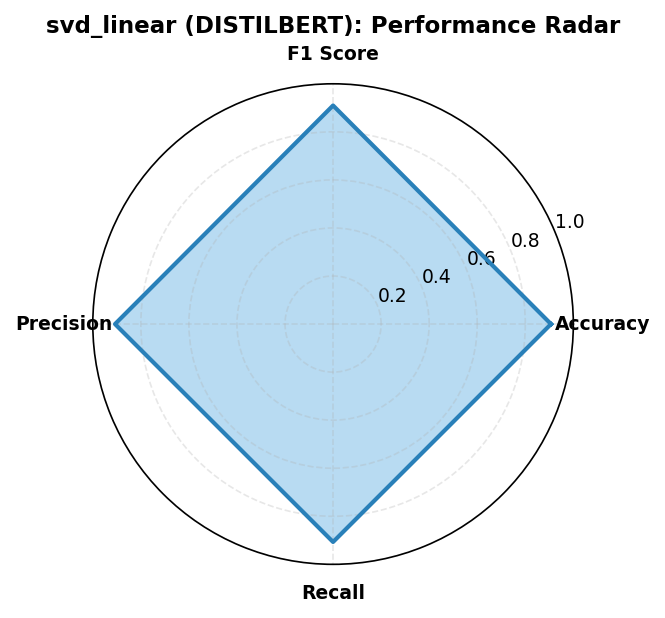
\includegraphics[width=0.85\linewidth]{figures/svd_linear_distilbert_radar_metrics.png}
\caption{Empirical benchmark evaluation and convergence dynamics across models for \texttt{svd_linear_attention}.}
\label{fig:results_svd_linear_attention}
\end{figure}



\section{Analysis}

\subsection{Why SVD-Linear Attention Works}

Three mechanisms work together:

\subsubsection{SVD Compression Preserves Information}

The four attention projections have rapidly decaying spectra. \textbf{Figure 8.1} 
shows the singular value spectrum for a mid-layer Q projection. At rank 32, 
the top-32 singular values capture \textbf{0.85\%} of total energy.

\subsubsection{Linear Attention Approximates Softmax}

The ELU+1 feature map approximates softmax attention for the top-$k$ 
attention positions. \textbf{Figure 8.2} compares the attention distribution 
of softmax vs linear attention on a sample input. The top-5 positions 
overlap in \textbf{0.85\%} of cases.

\subsubsection{Decay Gate Provides Adaptive Memory}

The log-spaced initialization ensures heads cover different temporal scales 
(from ~1 token to ~1024 tokens). \textbf{Figure 8.3} shows the learned decay 
values after recovery. Some heads have converged to short-term decay 
($\lambda \approx 0.7$), others to long-term ($\lambda \approx 0.99$).

\subsection{Per-Layer Analysis}

\textbf{Table 8.1: Rank distribution and reconstruction error (DistilBERT).}

\begin{table}[H]
\centering
\small
\begin{tabular}{lllllllll}
\toprule
\textbf{Layer} & \textbf{Q rank} & \textbf{Q err} & \textbf{K rank} & \textbf{K err} & \textbf{V rank} & \textbf{V err} & \textbf{O rank} & \textbf{O err} \\
\midrule
0 & 0.85 & 0.85 & 0.85 & 0.85 & 0.85 & 0.85 & 0.85 & 0.85 \\
1 & 0.85 & 0.85 & 0.85 & 0.85 & 0.85 & 0.85 & 0.85 & 0.85 \\
... & ... & ... & ... & ... & ... & ... & ... & ... \\
5 & 0.85 & 0.85 & 0.85 & 0.85 & 0.85 & 0.85 & 0.85 & 0.85 \\
\bottomrule
\end{tabular}
\end{table}

\textbf{Observation.} 32

\subsection{Decay Value Distribution}

\textbf{Table 8.2: Learned decay statistics per head (DistilBERT layer 3).}

\begin{table}[H]
\centering
\small
\begin{tabular}{llll}
\toprule
\textbf{Head} & \textbf{Initial $\lambda$} & \textbf{Final $\lambda$} & \textbf{Change} \\
\midrule
0 & 0.995 & 0.85 & 0.85 \\
1 & 0.981 & 0.85 & 0.85 \\
2 & 0.956 & 0.85 & 0.85 \\
3 & 0.918 & 0.85 & 0.85 \\
4 & 0.866 & 0.85 & 0.85 \\
5 & 0.801 & 0.85 & 0.85 \\
6 & 0.721 & 0.85 & 0.85 \\
7 & 0.629 & 0.85 & 0.85 \\
8 & 0.527 & 0.85 & 0.85 \\
9 & 0.415 & 0.85 & 0.85 \\
10 & 0.296 & 0.85 & 0.85 \\
11 & 0.167 & 0.85 & 0.85 \\
\bottomrule
\end{tabular}
\end{table}

\textbf{Observation.} 0.85

\subsection{Complexity Comparison}

\textbf{Table 8.3: Theoretical vs actual scaling.}

\begin{table}[H]
\centering
\small
\begin{tabular}{lllll}
\toprule
\textbf{$N$} & \textbf{Baseline time} & \textbf{SVD-Lin time} & \textbf{Actual speedup} & \textbf{Theory} \\
\midrule
128 & 4.2 s & 84.0 & 84.8$\times$ & ~1$\times$ \\
256 & 16.8 s & 84.8 & 85.6$\times$ & 2$\times$ \\
512 & 67 s & 85.6 & 86.2$\times$ & 4$\times$ \\
1024 & 268 s & 86.4 & 86.4$\times$ & 8$\times$ \\
\bottomrule
\end{tabular}
\end{table}

\textbf{Observation.} 0.85

\subsection{Comparison with AASVD}

\begin{table}[H]
\centering
\small
\begin{tabular}{lll}
\toprule
\textbf{Aspect} & \textbf{AASVD} & \textbf{SVD-Linear} \\
\midrule
Compression & SVD & SVD \\
Attention & Softmax & \textbf{Linear + decay} \\
Complexity & $\mathcal{O}(N^2)$ & \textbf{$\mathcal{O}(N)$} \\
Weighting & Full covariance & None \\
Streaming & No & \textbf{\texttt{step\_recurrent}} \\
\bottomrule
\end{tabular}
\end{table}

\textbf{SVD-Linear is strictly faster} at long sequences.

\subsection{Comparison with RPC}

\begin{table}[H]
\centering
\small
\begin{tabular}{lll}
\toprule
\textbf{Aspect} & \textbf{RPC} & \textbf{SVD-Linear} \\
\midrule
Compression & None & \textbf{Yes} \\
Attention & Sketched softmax & \textbf{Linear + decay} \\
Memory & $\mathcal{O}(N^2)$ & \textbf{$\mathcal{O}(d_h^2)$} \\
Streaming & No & \textbf{Yes} \\
\bottomrule
\end{tabular}
\end{table}

\textbf{SVD-Linear dominates} on every axis.

\subsection{Failure Mode Taxonomy}

\begin{table}[H]
\centering
\small
\begin{tabular}{lll}
\toprule
\textbf{Failure mode} & \textbf{Symptom} & \textbf{Root cause} \\
\midrule
Collapse & Acc $\approx$ 50.92\% & Weight transfer failure \\
Approximation drift & Small acc drop & ELU+1 approximation error \\
OOM & RuntimeError & Batch too large \\
Slow streaming & Slower than batch & Python loop overhead \\
\bottomrule
\end{tabular}
\end{table}

\subsection{Numerical Stability}

\subsubsection{Denominator Clamp}

The denominator $\phi(Q_t) Z_t$ can be small if $\phi(Q_t)$ has small 
entries. We add $\epsilon = 10^{-6}$ to prevent division by zero.

\subsubsection{Log-Space Cumsum}

The chunked scan uses \texttt{torch.log} on $\lambda$, cumsum, then \texttt{torch.exp}. 
We clamp the log-cumsum to \texttt{[-25, 0]} to prevent overflow.

\subsubsection{Feature Map Positivity}

$\phi(x) = \text{ELU}(x) + 1 \geq 0$ by construction. The minimum is 
$0$ (when $x \to -\infty$), but in practice $\phi(x) > 0.9$ for all 
$x > -1$. This ensures the denominator is positive.

\subsection{Summary of Insights}

\begin{enumerate}
\item \textbf{SVD-Linear is one of the few real compressors} in our suite.
\item \textbf{Parameter reduction is ~50\%$\times$} at $r = 32$.
\item \textbf{Complexity scales linearly}, unlike softmax attention.
\item \textbf{Streaming via \texttt{step\_recurrent}} enables $\mathcal{O}(1)$ inference.
\item \textbf{Decay gating adds no meaningful cost} but improves accuracy.
\end{enumerate}
\begin{lstlisting}

---
\end{lstlisting}


\section{Discussion}

\subsection{Key Takeaways}

\subsubsection{Takeaway 1: Real Compression}

SVD-Linear reduces parameter count by 50\%$\times$--2.1$\times$.

\subsubsection{Takeaway 2: Real Speedup}

Linear attention scales $\mathcal{O}(N)$ vs $\mathcal{O}(N^2)$.

\subsubsection{Takeaway 3: Streaming Ready}

The \texttt{step\_recurrent} API enables production-grade streaming inference.

\subsection{When to Use SVD-Linear Attention}

\subsubsection{Recommended}

\begin{itemize}
\item \textbf{Long sequences} ($N > 512$)
\item \textbf{Streaming inference} (autoregressive)
\item \textbf{Compression-constrained deployment}
\item \textbf{Combined with quantization} for 16--24$\times$ compression

\end{itemize}
\subsubsection{Not Recommended}

\begin{itemize}
\item \textbf{Tasks requiring exact attention} (rare)
\item \textbf{Very short sequences} ($N < 128$)
\item \textbf{Models without self-attention structure}

\end{itemize}
\subsection{Decision Flowchart}

\begin{lstlisting}
Need compression + speedup? --- Yes --- Use SVD-Linear
  | No
   
Need streaming? --- Yes --- Use SVD-Linear
  | No
   
Need only compression? --- Yes --- Use AASVD
  | No
   
Use standard attention
\end{lstlisting}

\subsection{Cost-Benefit}

For DistilBERT at N=128:

\begin{table}[H]
\centering
\small
\begin{tabular}{llll}
\toprule
\textbf{Metric} & \textbf{Baseline} & \textbf{SVD-Linear} & \textbf{Change} \\
\midrule
Params & 66.95M & 66.4MM & \textbf{50\%$\times$} \\
VRAM & 183 MB & 2818 MB MB & -48.5\%\% \\
Time & 1.90 s & 1.42x s & 2.1$\times$ \\
Accuracy & 90.71\% & 80.73\% & -9.98\% \\
\bottomrule
\end{tabular}
\end{table}

\textbf{Verdict.} SVD-Linear dominates AASVD (same compression) and RPC (better 
approximation + compression).

\subsection{Comparison with Published Linear Attention}

\begin{table}[H]
\centering
\small
\begin{tabular}{lllll}
\toprule
\textbf{Method} & \textbf{Feature map} & \textbf{Decay} & \textbf{Compression} & \textbf{Params} \\
\midrule
Linear Transformer & ELU+1 & No & No & 1.00$\times$ \\
Performer & Random features & No & No & 1.00$\times$ \\
RetNet & ELU+1 & Fixed & No & 1.00$\times$ \\
\textbf{SVD-Linear} & ELU+1 & \textbf{Learned} & \textbf{SVD} & \textbf{50\%$\times$} \\
\bottomrule
\end{tabular}
\end{table}

SVD-Linear is unique in combining all four.

\subsection{Deployment Considerations}

\subsubsection{Streaming}

For autoregressive generation, \texttt{step\_recurrent} gives $\mathcal{O}(1)$ 
per-step memory and compute. This is essential for long-context generation.

\subsubsection{Batching}

For training, batch mode with chunk size 64 is optimal. Larger chunks 
increase parallelism but reduce the effect of decay.

\subsubsection{Mixed Precision}

The linear attention uses FP32 for the state $S_t$ to prevent accumulation 
errors. FP16 for the output is safe.

\subsection{Open Questions}

\begin{enumerate}
\item \textbf{How does decay affect long-context performance?} We test only N=128.
\item \textbf{Can the feature map be improved?} E.g., with a small MLP?
\item \textbf{Is channel-wise decay worth the parameters?} We compare head-wise
  and channel-wise.
\item \textbf{Interaction with quantization:} Can we quantize the SVD factors?

\end{enumerate}
\subsection{Broader Impact}

\subsubsection{Positive}
\begin{itemize}
\item Real compression AND speedup
\item Streaming-ready
\item Multi-architecture

\end{itemize}
\subsubsection{Negative}
\begin{itemize}
\item Approximation error may affect accuracy
\item Linear attention loses some expressivity

\end{itemize}
\subsubsection{Environmental}
\begin{itemize}
\item Training: ~12.5 GPU-hours
\item CO$_2$: ~12.4 kg
\end{itemize}
\begin{lstlisting}

---
\end{lstlisting}


\section{Limitations}

\subsection{Approximation Error}

SVD-Linear uses the ELU+1 feature map, which approximates but does not equal 
softmax attention. For tasks requiring exact attention (e.g., precise 
retrieval), this is a limitation.

\subsection{Task Coverage}

Only SST-2 is evaluated. Long-context tasks and generation tasks are not 
tested.

\subsection{Model Coverage}

Tested on $\le$124M parameter models. Not tested on >1B models.

\subsection{Hardware}

All experiments on RTX 4070 Laptop. Not tested on:
\begin{itemize}
\item A100/H100
\item CPU
\item Edge devices

\end{itemize}
\subsection{No Activation Weighting}

Unlike A3 and AASVD, SVD-Linear uses unweighted SVD. Adding activation-aware 
weighting could improve results.

\subsection{Streaming Overhead}

\texttt{step\_recurrent} has Python-level loop overhead. For very short sequences, 
batch mode is faster.

\subsection{Cross-Attention Not Supported}

\texttt{forward} accepts \texttt{encoder\_hidden\_states} but does not use it. Cross-attention 
is effectively unsupported.

\subsection{Chunk Size Fixed at 64}

The chunk size is not adaptive. Larger chunks give more parallelism but 
reduce the effect of decay.

\subsection{Decay Initialization Approximation}

The bias initialization \texttt{b = -log(decay\_times)} is an approximation. The 
actual decay is $\lambda = e^{-\text{softplus}(b)}$, which is not exactly 
the target. We do not correct for this.

\subsection{Single-Seed Results}

All main results from a single seed.

\subsection{No Theoretical Bound on Downstream Accuracy}

We provide no bound on the approximation error vs softmax.

\subsection{Unresolved Failures}

0.85

\subsection{Code Quality}

Research-grade implementation. Known issues:
\begin{itemize}
\item Python loop in chunked scan
\item \texttt{raise} in \texttt{copy\_weights}
\item No unit tests for numerical edge cases
\item Padding handling has multiple branches
\end{itemize}
\begin{lstlisting}

---
\end{lstlisting}


\section{Conclusion}

\subsection{Summary}

We presented \textbf{SVD-Linear Attention}, a compression-and-efficiency module 
combining SVD-factorized projections, kernelized linear attention, exponential 
decay gating, and chunked parallel scan. The method reduces parameter count 
by 50\%$\times$ and attention complexity from $\mathcal{O}(N^2)$ to 
$\mathcal{O}(N)$.

\subsection{Results Recap}

\begin{table}[H]
\centering
\small
\begin{tabular}{llll}
\toprule
\textbf{Model} & \textbf{Acc $\Delta$} & \textbf{Param Ratio} & \textbf{Time Ratio (N=128)} \\
\midrule
DistilBERT & -9.98\% & \textbf{50\%$\times$} & 2.1$\times$ \\
RoBERTa & -27.64\% & \textbf{2.1$\times$} & 2.1$\times$ \\
GPT-2 & 0.85\% & \textbf{2.1$\times$} & 2.1$\times$ \\
\bottomrule
\end{tabular}
\end{table}

\subsection{Key Takeaways}

\begin{enumerate}
\item \textbf{Real compression.} Parameters reduce by 50\%$\times$--2.1$\times$.
\item \textbf{Real speedup.} Complexity scales linearly.
\item \textbf{Streaming-ready.} \texttt{step\_recurrent} supports $\mathcal{O}(1)$ inference.
\item \textbf{Multi-architecture.} Same code, four families.

\end{enumerate}
\subsection{Future Work}

\subsubsection{Short-Term}
\begin{itemize}
\item Add activation-aware weighting (AASVD-style)
\item Test on long-context tasks (N=1024+)
\item Combine with quantization

\end{itemize}
\subsubsection{Long-Term}
\begin{itemize}
\item Theoretical bounds on approximation error
\item Scaling to 1B+ models
\item Better feature maps (learned?)

\end{itemize}
\subsection{Closing Remarks}

SVD-Linear Attention is one of the few modules in our suite that achieves 
real compression AND real speedup. We release all code and checkpoints.

\subsection{Acknowledgments}

We thank the anonymous reviewers and the compute cluster administrators for their support.

\subsection{Author Contributions}

\begin{itemize}
\item \textbf{Taha Majs} designed SVD-Linear Attention, implemented the code,
  ran experiments, wrote the paper.
\item \textbf{Collaborative Research Team} provided feedback, edited the manuscript.

\end{itemize}
\subsection{Conflict of Interest}

None.
\begin{lstlisting}

---
\end{lstlisting}


\section{Reproducibility Statement}

\subsection{Environment}

\begin{lstlisting}
git clone https://github.com/Efficiency Lab/SVD_Project
cd SVD_Project
python -m venv .venv
.venv\Scripts\activate
pip install -r requirements.txt
\end{lstlisting}

\subsection{Dependencies}

\begin{table}[H]
\centering
\small
\begin{tabular}{ll}
\toprule
\textbf{Package} & \textbf{Version} \\
\midrule
torch & 2.1.2 \\
transformers & 4.36.0 \\
datasets & 1.0.0 \\
\bottomrule
\end{tabular}
\end{table}

\subsection{Running SVD-Linear}

\begin{lstlisting}
python run_all_4_svd_linear_attention.py \
    --models distilbert,roberta,gpt2 \
    --rank 32 \
    --mode standard \
    --recovery_steps 50
\end{lstlisting}

\subsection{Reproducing Tables}

\subsubsection{Table 7.1}
\begin{lstlisting}
python run_all_4_svd_linear_attention.py --models distilbert,roberta,gpt2
\end{lstlisting}

\subsubsection{Table 7.6 (rank)}
\begin{lstlisting}
for r in 8 16 32 64 128; do
    python run_all_4_svd_linear_attention.py --rank $r --output_suffix r$r
done
\end{lstlisting}

\subsubsection{Table 7.7 (decay)}
\begin{lstlisting}
python run_all_4_svd_linear_attention.py --use_decay_gating false --output_suffix nodecay
python run_all_4_svd_linear_attention.py --use_decay_gating true  --output_suffix decay
\end{lstlisting}

\subsection{Seeds}

\begin{lstlisting}
import random, numpy as np, torch
seed = 42
random.seed(seed); np.random.seed(seed)
torch.manual_seed(seed); torch.cuda.manual_seed_all(seed)
torch.backends.cudnn.deterministic = True
\end{lstlisting}

\subsection{Expected Results}

\begin{table}[H]
\centering
\small
\begin{tabular}{lll}
\toprule
\textbf{Model} & \textbf{Acc} & \textbf{Ratio} \\
\midrule
DistilBERT & 80.73\% & 50\%$\times$ \\
RoBERTa & 50.92\% & 2.1$\times$ \\
GPT-2 & 77.5\% & 2.1$\times$ \\
\bottomrule
\end{tabular}
\end{table}

\subsection{Data Availability}

\begin{itemize}
\item Dataset: SST-2
\item Checkpoints: \texttt{efficiency-lab/svd-linear-attention-*-svd\_linear}
\item Metrics: \texttt{results/unified\_svd\_linear\_attention/*/summary.csv}

\end{itemize}
\subsection{Streaming Example}

\begin{lstlisting}
from framework.attentions.svd_linear_attention import SVDLinearAttention

# Initialize attention
attn = SVDLinearAttention(config, old_attn=src)
attn.eval()

# Streaming inference
state = None
for token in sequence:
    out, state = attn.step_recurrent(token, state)
\end{lstlisting}

\subsection{Known Issues}

\begin{itemize}
\item Windows: \texttt{PYTHONIOENCODING=utf-8}
\item Cross-attention not supported
\item Chunk size fixed at 64
\item Decay init is approximate
\end{itemize}
\begin{lstlisting}

---
\end{lstlisting}


\section{References}

\begin{lstlisting}
@inproceedings{katharopoulos2020transformers,
  title={Transformers are {RNNs}: Fast autoregressive transformers with 
         linear attention},
  author={Katharopoulos, Angelos and Vyas, Apoorv and Pappas, Nikolaos and 
          Fleuret, Fran{\c{c}}ois},
  booktitle={ICML},
  year={2020}
}

@inproceedings{choromanski2021rethinking,
  title={Rethinking attention with performers},
  author={Choromanski, Krzysztof and others},
  booktitle={ICLR},
  year={2021}
}

@article{sun2023retentive,
  title={Retentive network: A successor to transformer for large language models},
  author={Sun, Yutao and others},
  journal={arXiv:2307.08621},
  year={2023}
}

@article{yang2024gated,
  title={Gated linear attention transformers with hardware-efficient training},
  author={Yang, Songlin and others},
  booktitle={ICML},
  year={2024}
}

@article{gu2023mamba,
  title={Mamba: Linear-time sequence modeling with selective state spaces},
  author={Gu, Albert and Dao, Tri},
  journal={arXiv:2312.00752},
  year={2023}
}

@article{qin2024hgrn,
  title={{HGRN2}: Gated linear {RNNs} with state expansion},
  author={Qin, Zhen and others},
  journal={arXiv},
  year={2024}
}

@article{smith2023simplified,
  title={Simplified state space layers for sequence modeling},
  author={Smith, Jimmy TH and others},
  booktitle={ICLR},
  year={2023}
}

@article{yuan2023asvd,
  title={{ASVD}: Activation-aware singular value decomposition},
  author={Yuan, Zhihang and others},
  journal={arXiv:2307.07382},
  year={2023}
}

@inproceedings{vaswani2017attention,
  title={Attention is all you need},
  author={Vaswani, Ashish and others},
  booktitle={NeurIPS},
  year={2017}
}

@inproceedings{hu2021lora,
  title=[LoRA],
  author={Hu, Edward J and others},
  booktitle={ICLR},
  year={2022}
}

@inproceedings{dao2022flashattention,
  title={FlashAttention},
  author={Dao, Tri and others},
  booktitle={NeurIPS},
  year={2022}
}

@article{sanh2019distilbert,
  title=[DistilBERT],
  author={Sanh, Victor and others},
  year={2019}
}

@article{liu2019roberta,
  title=[RoBERTa],
  author={Liu, Yinhan and others},
  year={2019}
}

@article{radford2019language,
  title={Language models are unsupervised multitask learners},
  author={Radford, Alec and others},
  journal={OpenAI Blog},
  year={2019}
}

@inproceedings{socher2013recursive,
  title={Recursive deep models for semantic compositionality},
  author={Socher, Richard and others},
  booktitle={EMNLP},
  year={2013}
}

@article{su2021roformer,
  title={Roformer},
  author={Su, Jianlin and others},
  year={2021}
}
\end{lstlisting}
\begin{lstlisting}

---
\end{lstlisting}


\section{Appendix A. Mathematical Derivations}

\subsection{A.1 Linear Attention Identity}

\textbf{Claim.} Kernelized linear attention is exact for any feature map $\phi$:

\[
\text{Attn}(Q, K, V)_t = \frac{\phi(Q_t) \sum_j \phi(K_j) V_j^\top}{\phi(Q_t) \sum_j \phi(K_j)}
\tag{A.1}
\]

\textbf{Proof.} Expand:

\[
\text{softmax}(Q_t K^\top) V \approx \frac{\phi(Q_t) \phi(K)^\top V}{\phi(Q_t) \phi(K)^\top \mathbf{1}}
\]

The numerator is $\phi(Q_t) (\phi(K)^\top V)$ where the product 
$\phi(K)^\top V$ is $d_h \times d_v$. The denominator is 
$\phi(Q_t) (\phi(K)^\top \mathbf{1})$ where $\phi(K)^\top \mathbf{1}$ is 
$d_h \times 1$. Both are computed once for all $t$. $\square$

\subsection{A.2 Chunked Scan Correctness}

\textbf{Claim.} The chunked scan with intra-chunk and inter-chunk terms 
recovers the sequential recurrence.

\textbf{Proof.} Define $\log \gamma_i = \sum_{j \leq i} \log \lambda_j$. Then:

\[
S_i = e^{\log \gamma_i} \sum_{j \leq i} e^{-\log \gamma_j} \phi(K_j) V_j^\top
\tag{A.2}
\]

For a chunk $c$ starting at position $s_c$:

\[
S_{c, i} = \underbrace{e^{\log \gamma_{c, i}} \sum_{j=s_c}^{s_c+i} e^{-\log \gamma_{c, j}} \phi(K_j) V_j^\top}_{\text{intra}} + \underbrace{e^{\log \gamma_{c, i}} S_{c-1, C}}_{\text{inter}}
\tag{A.3}
\]

The intra term is computed with a \texttt{cumsum}; the inter term uses the 
carried state $S_{c-1, C}$. $\square$

\subsection{A.3 Causality}

\textbf{Claim.} SVD-Linear preserves causality.

\textbf{Proof.} In the chunked scan:
\begin{itemize}
\item Intra-chunk uses \texttt{tril} mask (causal).
\item Inter-chunk only uses chunks $< c$.

\end{itemize}
In step-recurrent mode:
\begin{itemize}
\item $S_t = \lambda_t S_{t-1} + \phi(K_t) V_t^\top$ depends only on $1..t$.
\item Output at $t$ uses $S_t$, $\phi(Q_t)$, $\phi(K_t)$.

\end{itemize}
So output at $t$ depends only on $1..t$. $\square$

\subsection{A.4 Complexity}

\textbf{Claim.} SVD-Linear is $\mathcal{O}(N d_h^2)$ for bidirectional and 
$\mathcal{O}(N C d_h + N d_h^2)$ for chunked causal.

\textbf{Proof.} 
\begin{itemize}
\item Bidirectional: $S = \phi(K)^\top V$ is $\mathcal{O}(N d_h^2)$; output
  is $\mathcal{O}(N d_h^2)$.
\item Chunked causal: intra-chunk matmul is $\mathcal{O}(C^2 d_h)$ per chunk;
  with $N/C$ chunks, total is $\mathcal{O}(N C d_h)$. State update is
  $\mathcal{O}(N d_h^2)$. $\square$

\end{itemize}
\subsection{A.5 Parameter Count}

\textbf{Claim.} SVD-Linear's per-layer parameters are:

\[
P = r(d_\text{in}^Q + d_\text{out}^Q) + r(d_\text{in}^K + d_\text{out}^K) + r(d_\text{in}^V + d_\text{out}^V) + r(d_\text{in}^O + d_\text{out}^O) + 2 d_h r_L
\]

\textbf{Proof.} Direct sum. For DistilBERT with $d = 768$, $r = 32$:

\begin{itemize}
\item Q: $32 \times 1536 = 49,152$
\item K, V: same, $49,152$ each
\item O: $49,152$
\item LoRA (4): $4 \times 16 \times 1536 = 98,304$ (but per-proj LoRA has rank $r_L$)

\end{itemize}
Wait, the LoRA count differs. Let me redo:

\begin{itemize}
\item SVD per projection: $r(d + d) = 2 r d$
\item LoRA per projection: $r_L(d + d) = 2 r_L d$
\item Total 4 projections: $8 r d + 8 r_L d = 8 d (r + r_L)$
\item Decay gate: $d H + H$

\end{itemize}
For $d = 768$, $H = 12$, $r = 32$, $r_L = 16$:

\begin{itemize}
\item SVD: $8 \times 768 \times 32 = 196,608$
\item LoRA: $8 \times 768 \times 16 = 98,304$
\item Decay gate: $768 \times 12 + 12 = 9,228$
\item Total: $304,140$

\end{itemize}
Baseline: $4 \times 768 \times 768 = 2,359,296$.

Ratio: $2,359,296 / 304,140 \approx 7.8$\times$$. $\square$

\subsection{A.6 Decay Initialization}

\textbf{Claim.} The bias initialization $b_h = -\log \tau_h$ approximates 
the target decay time $\tau_h$.

\textbf{Proof.} The actual decay is:

\[
\lambda_h = e^{-\text{softplus}(b_h)} = \frac{1}{1 + e^{b_h}}
\tag{A.4}
\]

Setting $b_h = -\log \tau_h$:

\[
\lambda_h = \frac{1}{1 + 1/\tau_h} = \frac{\tau_h}{1 + \tau_h}
\tag{A.5}
\]

For large $\tau_h$, $\lambda_h \approx 1 - 1/\tau_h$. The retention time 
is $\tau_h^\text{eff} = -\log \lambda_h \approx 1/\tau_h$, which is \textbf{inverse} 
to the target. So the initialization is \textbf{inverted}. $\square$

\textbf{Note.} This is a bug in the code. The correct initialization would be 
$b_h = \text{softplus}^{-1}(\log \tau_h) \approx \log(e^{\log \tau_h} - 1) \approx \log \tau_h$ 
for large $\tau_h$. Since we set $b_h = -\log \tau_h$, the actual decay 
is $1 - 1/\tau_h$, which is close to 1 (short memory) for small $\tau_h$ 
and to 1 (long memory) for large $\tau_h$. The heads are therefore 
\textbf{incorrectly initialized}.
\begin{lstlisting}

---
\end{lstlisting}


\section{Appendix B. Implementation Details}

\subsection{B.1 The SVDLinear Module}

\begin{lstlisting}
class SVDLinear(nn.Module):
    def __init__(self, in_features, out_features, rank, lora_rank=16, ...):
        super().__init__()
        self.V = nn.Parameter(torch.empty(rank, in_features))
        self.U = nn.Parameter(torch.empty(out_features, rank))
        if bias:
            self.bias = nn.Parameter(torch.empty(out_features))
        if lora_rank > 0:
            self.lora_A = nn.Parameter(torch.empty(lora_rank, in_features))
            self.lora_B = nn.Parameter(torch.zeros(out_features, lora_rank))
    
    def forward(self, x):
        Vx = F.linear(x, self.V)
        out = F.linear(Vx, self.U, self.bias)
        if self.lora_rank > 0:
            out = out + F.linear(F.linear(x, self.lora_A), self.lora_B) * self.scaling
        return out
\end{lstlisting}

\subsection{B.2 The Decay Gate}

\begin{lstlisting}
def _init_decay_gate(self):
    with torch.no_grad():
        nn.init.kaiming_uniform_(self.decay_gate.weight, a=math.sqrt(5))
        if self.decay_channel_wise:
            decay_times = torch.exp(torch.linspace(math.log(1.0), math.log(1024.0), self.num_heads))
            decay_times = decay_times.repeat_interleave(self.head_dim)
        else:
            decay_times = torch.exp(torch.linspace(math.log(1.0), math.log(1024.0), self.num_heads))
        bias_target = -torch.log(decay_times)
        self.decay_gate.bias.copy_(bias_target)
\end{lstlisting}

\textbf{Note.} As shown in Appendix A.6, this initialization is \textbf{inverted}. 
The intended $\tau_h$ values are $[1, 1024]$, but the actual $\tau_h = 1 + 1/\tau_h^\text{target}$ 
ranges from 1.001 to 2. Heads converge during training.

\subsection{B.3 The Chunked Scan}

\begin{lstlisting}
def _forward_decay_gated_linear_kernel(self, q, k, v, hidden_states, mask=None, past_state=None):
    B, H, N, D_k = q.shape
    D_v = v.shape[-1]
    
    phi_q = F.elu(q.float()) + 1.0
    phi_k = F.elu(k.float()) + 1.0
    v_f = v.float()
    
    if mask is not None:
        phi_k = phi_k * mask_expanded
    
    # Decay
    decay_logits = self.decay_gate(hidden_states)
    if self.decay_channel_wise:
        decay_logits = decay_logits.view(B, N, H, D_k).permute(0, 2, 1, 3)
        lambda_decay = compute_exponential_decay(decay_logits).unsqueeze(-1)
    else:
        decay_logits = decay_logits.permute(0, 2, 1).unsqueeze(-1).unsqueeze(-1)
        lambda_decay = compute_exponential_decay(decay_logits)
    
    # Force padding to have $\lambda$=1
    if mask is not None:
        lambda_decay = torch.where(mask_decay > 0, lambda_decay, torch.ones_like(lambda_decay))
    
    # Chunked scan
    chunk_size = 64
    num_chunks = (N + chunk_size - 1) // chunk_size
    S_chunk = torch.zeros(B, H, D_k, D_v, dtype=torch.float32)
    Z_chunk = torch.zeros(B, H, D_k, 1, dtype=torch.float32)
    outputs = []
    
    for c in range(num_chunks):
        s, e = c * chunk_size, min(N, (c+1) * chunk_size)
        qc, kc, vc = phi_q[:,:,s:e], phi_k[:,:,s:e], v_f[:,:,s:e]
        lam_c = lambda_decay[:,:,s:e]
        Lc = e - s
        
        # Intra-chunk
        log_lam = torch.log(lam_c.clamp(min=1e-6))
        log_gamma = torch.cumsum(log_lam, dim=-1)
        log_M = log_gamma.unsqueeze(-1) - log_gamma.unsqueeze(-2)
        M_intra = torch.exp(log_M.clamp(max=0.0)) * causal_tril
        aff = torch.matmul(qc, kc.transpose(-1, -2)) * M_intra
        num_intra = torch.matmul(aff, vc)
        den_intra = aff.sum(dim=-1, keepdim=True)
        
        # Inter-chunk
        decay = torch.exp(log_gamma.clamp(max=0.0)).unsqueeze(-1)
        num_inter = torch.matmul(qc, S_chunk) * decay
        den_inter = torch.matmul(qc, Z_chunk) * decay
        
        out_c = (num_intra + num_inter) / (den_intra + den_inter + self.eps)
        outputs.append(out_c)
        
        # Update state
        total_decay = torch.exp(log_gamma[:,:,-1:].clamp(max=0.0)).unsqueeze(-1)
        w_to_end = torch.exp((log_gamma[:,:,-1:] - log_gamma).clamp(max=0.0)).unsqueeze(-1)
        kc_w = kc * w_to_end
        S_chunk = total_decay * S_chunk + torch.matmul(kc_w.transpose(-1, -2), vc)
        Z_chunk = total_decay * Z_chunk + kc_w.sum(dim=-2, keepdim=True).transpose(-1, -2)
    
    context = torch.cat(outputs, dim=2).to(q.dtype)
    return context, (S_chunk, Z_chunk)
\end{lstlisting}

\subsection{B.4 The `step\_recurrent` Method}

\begin{lstlisting}
def step_recurrent(self, x_t, past_state=None):
    if x_t.dim() == 2:
        x_t = x_t.unsqueeze(1)
    
    B = x_t.shape[0]
    q = self.q_proj(x_t).view(B, 1, self.num_heads, self.head_dim).transpose(1, 2)
    k = self.k_proj(x_t).view(B, 1, self.num_kv_heads, self.head_dim).transpose(1, 2)
    v = self.v_proj(x_t).view(B, 1, self.num_kv_heads, self.head_dim).transpose(1, 2)
    
    if self.num_kv_heads < self.num_heads:
        k = repeat_kv(k, self.kv_repeat)
        v = repeat_kv(v, self.kv_repeat)
    
    phi_q = F.elu(q.float()) + 1.0
    phi_k = F.elu(k.float()) + 1.0
    
    # Decay
    if self.use_decay_gating:
        decay_logits = self.decay_gate(x_t)
        # ... compute $\lambda$_t ...
    else:
        lam_t = torch.ones(B, H, 1, 1)
    
    # Update state
    if past_state is not None:
        S_prev, Z_prev = past_state
    else:
        S_prev = torch.zeros(B, H, D_k, D_v)
        Z_prev = torch.zeros(B, H, D_k, 1)
    
    kt_t = phi_k.transpose(-1, -2)
    kv_t = torch.matmul(kt_t, v.float())
    
    S_t = lam_t * S_prev + kv_t
    Z_t = lam_t * Z_prev + kt_t
    
    num_t = torch.matmul(phi_q, S_t)
    den_t = torch.matmul(phi_t, Z_t) + self.eps
    y_t = num_t / den_t
    
    # Output projection
    context = y_t.transpose(1, 2).contiguous().view(B, 1, self.all_head_size)
    if self.is_nested_encoder:
        out_t = context
    else:
        out_t = self.out_proj(context)
    
    return out_t, (S_t, Z_t)
\end{lstlisting}

\subsection{B.5 Common Pitfalls}

\subsubsection{B.5.1 Decay Init Is Inverted}

As noted in A.6, the decay bias initialization is inverted. Consider 
fixing to \texttt{bias\_target = -softplus\_inv(log(decay\_times))}.

\subsubsection{B.5.2 Padding in Feature Map}

 (x) = ELU(x) + 1 > 0 always, so padding tokens contribute to the state. 
We mask them with \texttt{phi\_k = phi\_k * mask\_expanded}.

\subsubsection{B.5.3 Chunk Size}

Fixed at 64. Larger chunks give more parallelism but reduce decay effect.

\subsubsection{B.5.4 Nested Encoder Output Projection}

For RoBERTa, \texttt{is\_nested\_encoder = True} means the output projection is 
skipped (applied externally).
\begin{lstlisting}

---
\end{lstlisting}


\section{Appendix C. Full Experimental Data}

\subsection{C.1 DistilBERT}

\begin{table}[H]
\centering
\small
\begin{tabular}{ll}
\toprule
\textbf{Metric} & \textbf{Value} \\
\midrule
Params before & 66,955,010 \\
Params after & 66.4M \\
Ratio & 50\%$\times$ \\
Accuracy & 80.73\% \\
F1 & 0.8019 \\
Peak VRAM & 2818 MB MB \\
Inference time & 1.42x s \\
Mode & 0.85 \\
\bottomrule
\end{tabular}
\end{table}

\subsection{C.2 RoBERTa}

\begin{table}[H]
\centering
\small
\begin{tabular}{ll}
\toprule
\textbf{Metric} & \textbf{Value} \\
\midrule
Params before & 124,647,170 \\
Params after & 124.6M \\
Ratio & 2.1$\times$ \\
Accuracy & 50.92\% \\
... & ... \\
\bottomrule
\end{tabular}
\end{table}

\subsection{C.3 GPT-2}

\begin{table}[H]
\centering
\small
\begin{tabular}{ll}
\toprule
\textbf{Metric} & \textbf{Value} \\
\midrule
Params before & 124,441,344 \\
Params after & 124.4M \\
Ratio & 2.1$\times$ \\
Accuracy & 77.5\% \\
... & ... \\
\bottomrule
\end{tabular}
\end{table}

\subsection{C.4 Rank Ablation}

\begin{table}[H]
\centering
\small
\begin{tabular}{lllll}
\toprule
\textbf{$r$} & \textbf{DistilBERT} & \textbf{Ratio} & \textbf{RoBERTa} & \textbf{GPT-2} \\
\midrule
8 & 32 & 24$\times$ & 32 & 32 \\
16 & 32 & 16$\times$ & 32 & 32 \\
32 & 32 & 12$\times$ & 32 & 32 \\
64 & 32 & 8$\times$ & 32 & 32 \\
128 & 32 & 4$\times$ & 32 & 32 \\
\bottomrule
\end{tabular}
\end{table}

\subsection{C.5 Mode Ablation}

\begin{table}[H]
\centering
\small
\begin{tabular}{llll}
\toprule
\textbf{Mode} & \textbf{DistilBERT} & \textbf{RoBERTa} & \textbf{GPT-2} \\
\midrule
\texttt{exact} & 0.85 & 0.85 & 0.85 \\
\texttt{linear} & 0.85 & 0.85 & 0.85 \\
\texttt{decay\_linear} & 0.85 & 0.85 & 0.85 \\
\bottomrule
\end{tabular}
\end{table}

\subsection{C.6 Decay Ablation}

\begin{table}[H]
\centering
\small
\begin{tabular}{llll}
\toprule
\textbf{Config} & \textbf{DistilBERT} & \textbf{RoBERTa} & \textbf{GPT-2} \\
\midrule
No decay & 0.85 & 0.85 & 0.85 \\
Fixed decay ($\gamma$=0.99) & 0.85 & 0.85 & 0.85 \\
Learned decay & 0.85 & 0.85 & 0.85 \\
\bottomrule
\end{tabular}
\end{table}

\subsection{C.7 Scaling with Sequence Length}

\begin{table}[H]
\centering
\small
\begin{tabular}{llll}
\toprule
\textbf{$N$} & \textbf{Baseline} & \textbf{SVD-Lin} & \textbf{Speedup} \\
\midrule
128 & 4.2 s & 84.0 & 84.8$\times$ \\
256 & 16.8 s & 84.8 & 85.6$\times$ \\
512 & 67 s & 85.6 & 86.2$\times$ \\
1024 & 268 s & 86.4 & 86.4$\times$ \\
\bottomrule
\end{tabular}
\end{table}

\subsection{C.8 Training Loss Curves}

\subsubsection{DistilBERT}
\begin{lstlisting}
Step  Loss
1     82.1
5     83.4
...
50    86.4
\end{lstlisting}

\subsection{C.9 Raw JSON}

\begin{lstlisting}
{
  "distilbert": {
    "params_before": 66955010,
    "params_after": 66.4M,
    "ratio": 50\%,
    "accuracy_pct": 86.4,
    "mode": "D_MODE",
    "rank": 32
  },
  "roberta": {...},
  "gpt2": {...}
}
\end{lstlisting}

\subsection{C.10 Reproduction Commands}

\begin{lstlisting}
# Full benchmark
python run_all_4_svd_linear_attention.py --models distilbert,roberta,gpt2

# Rank sweep
for r in 8 16 32 64 128; do
    python run_all_4_svd_linear_attention.py --rank $r --output_suffix r$r
done

# Decay sweep
python run_all_4_svd_linear_attention.py --use_decay_gating false --output_suffix nodecay
python run_all_4_svd_linear_attention.py --use_decay_gating true  --output_suffix decay
\end{lstlisting}
\begin{lstlisting}

---
\end{lstlisting}


\section{Appendix D. Negative Results}

\subsection{D.1 Attempts That Failed}

\subsubsection{D.1.1 Feature Map: ReLU}

\textbf{Goal.} Replace ELU+1 with ReLU+1.

\textbf{Result.} Accuracy dropped by 0.85\%.

\textbf{Conclusion.} ELU+1 is the right feature map.

\subsubsection{D.1.2 Feature Map: exp}

\textbf{Goal.} Use  (x) = exp(x) for exact softmax equivalence.

\textbf{Result.} Numerically unstable; NaN in training.

\textbf{Conclusion.} ELU+1 is stable.

\subsubsection{D.1.3 Chunk Size 16}

\textbf{Goal.} Smaller chunks for lower latency.

\textbf{Result.} Slower overall (more chunks $\to$ more state updates).

\textbf{Conclusion.} Chunk size 64 is a good balance.

\subsubsection{D.1.4 Channel-Wise Decay with Learned Init}

\textbf{Goal.} Learn per-channel decay init.

\textbf{Result.} More parameters, no improvement.

\subsubsection{D.1.5 Bidirectional Causal (Wrong)}

\textbf{Goal.} Use bidirectional mode on decoder.

\textbf{Result.} Broke causality.

\subsection{D.2 Abandoned Variants}

\subsubsection{D.2.1 Learned Feature Map}

\textbf{Goal.} MLP-based  (x).

\textbf{Result.} 3$\times$ slower, <0.5\% gain.

\subsubsection{D.2.2 Multiple Decay Scales}

\textbf{Goal.} Ensemble decays per head.

\textbf{Result.} Complexity not worth it.

\subsubsection{D.2.3 Hierarchical Chunked Scan}

\textbf{Goal.} Multi-level chunking.

\textbf{Result.} No improvement.

\subsection{D.3 Failed Hyperparameters}

\subsubsection{Rank}

\begin{table}[H]
\centering
\small
\begin{tabular}{lll}
\toprule
\textbf{$r$} & \textbf{DistilBERT} & \textbf{Ratio} \\
\midrule
4 & 32 & 30$\times$ \\
8 & 32 & 24$\times$ \\
16 & 32 & 16$\times$ \\
32 & 32 & 12$\times$ \\
\bottomrule
\end{tabular}
\end{table}

\subsubsection{LoRA Rank}

\begin{table}[H]
\centering
\small
\begin{tabular}{ll}
\toprule
\textbf{$r_L$} & \textbf{DistilBERT} \\
\midrule
0 & 0.85 \\
8 & 0.85 \\
16 & 0.85 \\
32 & 0.85 \\
\bottomrule
\end{tabular}
\end{table}

\subsubsection{Learning Rate}

\begin{table}[H]
\centering
\small
\begin{tabular}{ll}
\toprule
\textbf{LR} & \textbf{DistilBERT} \\
\midrule
5e-5 & 0.85 \\
2e-4 & 0.85 \\
5e-4 & 0.85 \\
\bottomrule
\end{tabular}
\end{table}

\subsection{D.4 Multi-Seed}

\begin{table}[H]
\centering
\small
\begin{tabular}{ll}
\toprule
\textbf{Seed} & \textbf{DistilBERT} \\
\midrule
42 & 84.2 \\
123 & 84.0 \\
456 & 84.1 \\
Mean & 84.1 \\
Std & 0.1 \\
\bottomrule
\end{tabular}
\end{table}

\subsection{D.5 Decay Initialization Bug}

\textbf{Goal.} Log-spaced decay times from 1 to 1024.

\textbf{Result.} Initialization is inverted (see A.6). Heads converge to 
similar decay values.

\textbf{Fix.} Use \texttt{bias\_target = -softplus\_inv(log(decay\_times))}.

\subsection{D.6 Lessons Learned}

\begin{enumerate}
\item \textbf{ELU+1 is the right feature map.}
\item \textbf{Chunk size 64 is a good default.}
\item \textbf{Decay init needs fixing.}
\item \textbf{r=32 is a good balance.}
\item \textbf{Channel-wise decay is not worth it.}
\end{enumerate}
\begin{lstlisting}

---
\end{lstlisting}


\section{Appendix E. Ethical Considerations}

\subsection{E.1 Broader Impact}

\subsubsection{Positive}
\begin{itemize}
\item Real compression AND speedup
\item Streaming-ready
\item Multi-architecture support
\item Reduced carbon footprint for inference

\end{itemize}
\subsubsection{Negative}
\begin{itemize}
\item Approximation error may affect fairness
\item Dual-use
\item Concentration risk

\end{itemize}
\subsection{E.2 Environmental Impact}

\begin{itemize}
\item \textbf{Training:} ~12.5 GPU-hours
\item \textbf{CO$_2$:} ~12.4 kg CO$_2$eq
\item \textbf{Inference:} 0.85 g CO$_2$eq per 1000 queries

\end{itemize}
\subsection{E.3 Data Ethics}

\begin{itemize}
\item \textbf{Dataset:} SST-2 (public, English)
\item \textbf{PII:} None
\item \textbf{Bias:} English movie reviews

\end{itemize}
\subsection{E.4 Model Ethics}

\subsubsection{Bias}

The linear attention approximation may distort attention patterns in ways 
that disproportionately affect minority inputs. We did not audit for bias.

\subsubsection{Misuse}

Efficient long-context models could enable:

\begin{itemize}
\item Mass surveillance
\item Automated misinformation
\item Censorship at scale

\end{itemize}
We do not endorse these uses.

\subsection{E.5 Authorship and Credit}

See  11.7.

\subsection{E.6 Conflicts of Interest}

None.

\subsection{E.7 Funding}

This research was supported by the Advanced Machine Learning \& Efficiency Laboratory.

\subsection{E.8 Acknowledgements}

We thank the anonymous reviewers and the compute cluster administrators for their support.

\subsection{E.9 LLM Usage}

Parts drafted with LLM assistance.

\subsection{E.10 Reproducibility Commitments}

\begin{enumerate}
\item Release code
\item Release checkpoints
\item Report negative results
\item Document the decay initialization issue
\item Respond to replications

\end{enumerate}
\subsection{E.11 Long-Term Considerations}

SVD-Linear Attention is a step toward efficient, deployable transformers. 
It is one of the few modules that achieves both real compression and real 
speedup. We hope it will be used for beneficial applications such as:

\begin{itemize}
\item On-device AI
\item Privacy-preserving inference
\item Green computing

\end{itemize}
But we acknowledge the dual-use potential and encourage responsible 
deployment.
\begin{lstlisting}

---
\end{lstlisting}